% Created by tikzDevice version 0.10.1 on 2017-10-30 17:28:46
% !TEX encoding = UTF-8 Unicode
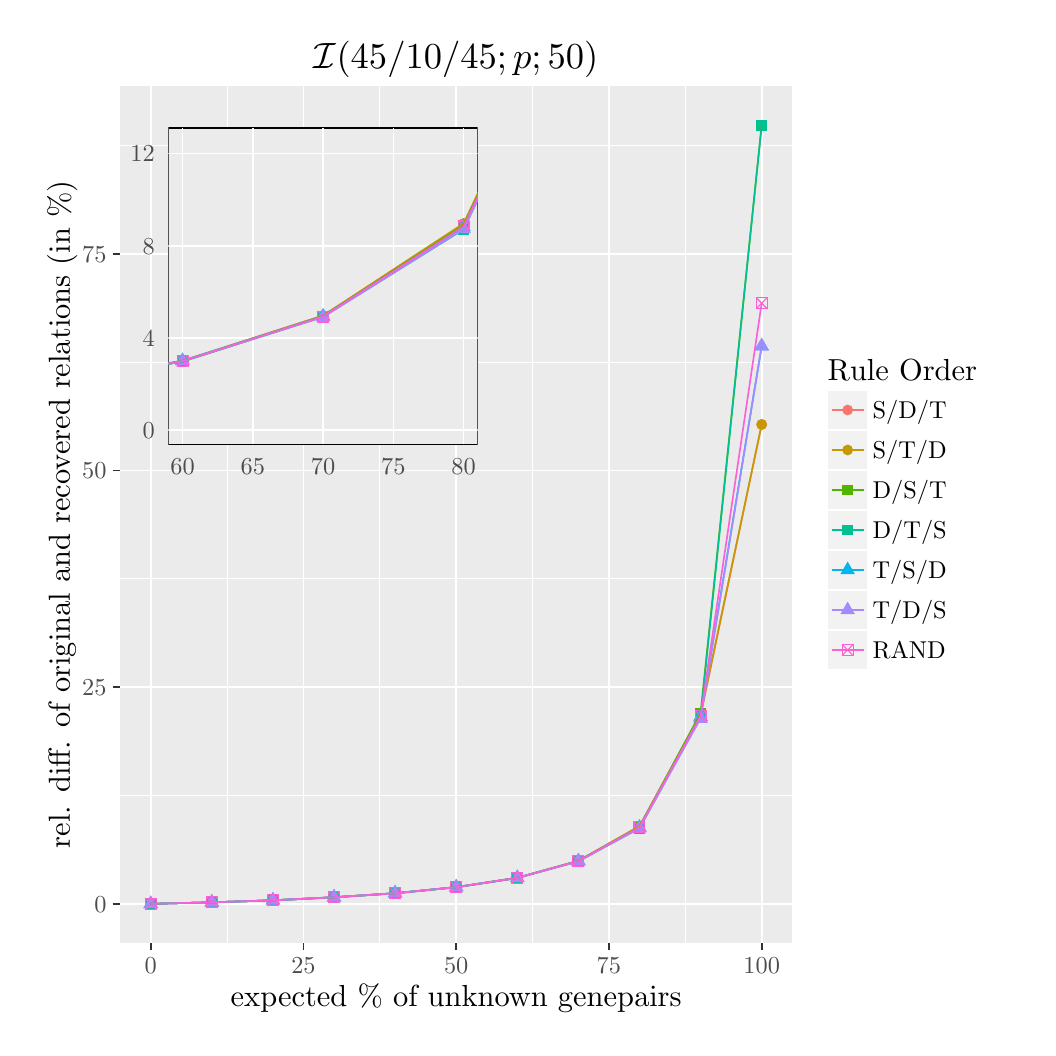
\begin{tikzpicture}[x=1pt,y=1pt]
\definecolor{fillColor}{RGB}{255,255,255}
\path[use as bounding box,fill=fillColor,fill opacity=0.00] (0,0) rectangle (361.35,361.35);
\begin{scope}
\path[clip] (  0.00,  0.00) rectangle (361.35,361.35);
\definecolor{drawColor}{RGB}{255,255,255}
\definecolor{fillColor}{RGB}{255,255,255}

\path[draw=drawColor,line width= 0.6pt,line join=round,line cap=round,fill=fillColor] (  0.00,  0.00) rectangle (361.35,361.35);
\end{scope}
\begin{scope}
\path[clip] ( 33.42, 30.69) rectangle (276.26,340.16);
\definecolor{fillColor}{gray}{0.92}

\path[fill=fillColor] ( 33.42, 30.69) rectangle (276.26,340.16);
\definecolor{drawColor}{RGB}{255,255,255}

\path[draw=drawColor,line width= 0.3pt,line join=round] ( 33.42, 83.91) --
	(276.26, 83.91);

\path[draw=drawColor,line width= 0.3pt,line join=round] ( 33.42,162.21) --
	(276.26,162.21);

\path[draw=drawColor,line width= 0.3pt,line join=round] ( 33.42,240.52) --
	(276.26,240.52);

\path[draw=drawColor,line width= 0.3pt,line join=round] ( 33.42,318.83) --
	(276.26,318.83);

\path[draw=drawColor,line width= 0.3pt,line join=round] ( 72.06, 30.69) --
	( 72.06,340.16);

\path[draw=drawColor,line width= 0.3pt,line join=round] (127.25, 30.69) --
	(127.25,340.16);

\path[draw=drawColor,line width= 0.3pt,line join=round] (182.44, 30.69) --
	(182.44,340.16);

\path[draw=drawColor,line width= 0.3pt,line join=round] (237.63, 30.69) --
	(237.63,340.16);

\path[draw=drawColor,line width= 0.6pt,line join=round] ( 33.42, 44.75) --
	(276.26, 44.75);

\path[draw=drawColor,line width= 0.6pt,line join=round] ( 33.42,123.06) --
	(276.26,123.06);

\path[draw=drawColor,line width= 0.6pt,line join=round] ( 33.42,201.37) --
	(276.26,201.37);

\path[draw=drawColor,line width= 0.6pt,line join=round] ( 33.42,279.67) --
	(276.26,279.67);

\path[draw=drawColor,line width= 0.6pt,line join=round] ( 44.46, 30.69) --
	( 44.46,340.16);

\path[draw=drawColor,line width= 0.6pt,line join=round] ( 99.65, 30.69) --
	( 99.65,340.16);

\path[draw=drawColor,line width= 0.6pt,line join=round] (154.84, 30.69) --
	(154.84,340.16);

\path[draw=drawColor,line width= 0.6pt,line join=round] (210.03, 30.69) --
	(210.03,340.16);

\path[draw=drawColor,line width= 0.6pt,line join=round] (265.23, 30.69) --
	(265.23,340.16);
\definecolor{fillColor}{RGB}{248,118,109}

\path[fill=fillColor] ( 44.46, 44.75) circle (  1.96);

\path[fill=fillColor] ( 66.54, 45.30) circle (  1.96);

\path[fill=fillColor] ( 88.61, 46.02) circle (  1.96);

\path[fill=fillColor] (110.69, 47.11) circle (  1.96);

\path[fill=fillColor] (132.77, 48.58) circle (  1.96);

\path[fill=fillColor] (154.84, 50.77) circle (  1.96);

\path[fill=fillColor] (176.92, 54.12) circle (  1.96);

\path[fill=fillColor] (199.00, 60.31) circle (  1.96);

\path[fill=fillColor] (221.07, 72.76) circle (  1.96);

\path[fill=fillColor] (243.15,112.65) circle (  1.96);

\path[fill=fillColor] (265.23,217.96) circle (  1.96);
\definecolor{fillColor}{RGB}{196,154,0}

\path[fill=fillColor] ( 44.46, 44.75) circle (  1.96);

\path[fill=fillColor] ( 66.54, 45.30) circle (  1.96);

\path[fill=fillColor] ( 88.61, 46.04) circle (  1.96);

\path[fill=fillColor] (110.69, 47.16) circle (  1.96);

\path[fill=fillColor] (132.77, 48.60) circle (  1.96);

\path[fill=fillColor] (154.84, 50.80) circle (  1.96);

\path[fill=fillColor] (176.92, 54.19) circle (  1.96);

\path[fill=fillColor] (199.00, 60.32) circle (  1.96);

\path[fill=fillColor] (221.07, 72.84) circle (  1.96);

\path[fill=fillColor] (243.15,113.36) circle (  1.96);

\path[fill=fillColor] (265.23,217.96) circle (  1.96);
\definecolor{fillColor}{RGB}{83,180,0}

\path[fill=fillColor] ( 42.50, 42.79) --
	( 46.42, 42.79) --
	( 46.42, 46.72) --
	( 42.50, 46.72) --
	cycle;

\path[fill=fillColor] ( 64.58, 43.33) --
	( 68.50, 43.33) --
	( 68.50, 47.26) --
	( 64.58, 47.26) --
	cycle;

\path[fill=fillColor] ( 86.65, 44.04) --
	( 90.58, 44.04) --
	( 90.58, 47.96) --
	( 86.65, 47.96) --
	cycle;

\path[fill=fillColor] (108.73, 45.13) --
	(112.65, 45.13) --
	(112.65, 49.06) --
	(108.73, 49.06) --
	cycle;

\path[fill=fillColor] (130.81, 46.60) --
	(134.73, 46.60) --
	(134.73, 50.52) --
	(130.81, 50.52) --
	cycle;

\path[fill=fillColor] (152.88, 48.77) --
	(156.81, 48.77) --
	(156.81, 52.69) --
	(152.88, 52.69) --
	cycle;

\path[fill=fillColor] (174.96, 52.12) --
	(178.88, 52.12) --
	(178.88, 56.04) --
	(174.96, 56.04) --
	cycle;

\path[fill=fillColor] (197.03, 58.25) --
	(200.96, 58.25) --
	(200.96, 62.17) --
	(197.03, 62.17) --
	cycle;

\path[fill=fillColor] (219.11, 70.61) --
	(223.03, 70.61) --
	(223.03, 74.54) --
	(219.11, 74.54) --
	cycle;

\path[fill=fillColor] (241.19,111.71) --
	(245.11,111.71) --
	(245.11,115.63) --
	(241.19,115.63) --
	cycle;

\path[fill=fillColor] (263.26,324.13) --
	(267.19,324.13) --
	(267.19,328.05) --
	(263.26,328.05) --
	cycle;
\definecolor{fillColor}{RGB}{0,192,148}

\path[fill=fillColor] ( 42.50, 42.79) --
	( 46.42, 42.79) --
	( 46.42, 46.72) --
	( 42.50, 46.72) --
	cycle;

\path[fill=fillColor] ( 64.58, 43.33) --
	( 68.50, 43.33) --
	( 68.50, 47.25) --
	( 64.58, 47.25) --
	cycle;

\path[fill=fillColor] ( 86.65, 44.04) --
	( 90.58, 44.04) --
	( 90.58, 47.97) --
	( 86.65, 47.97) --
	cycle;

\path[fill=fillColor] (108.73, 45.12) --
	(112.65, 45.12) --
	(112.65, 49.04) --
	(108.73, 49.04) --
	cycle;

\path[fill=fillColor] (130.81, 46.59) --
	(134.73, 46.59) --
	(134.73, 50.51) --
	(130.81, 50.51) --
	cycle;

\path[fill=fillColor] (152.88, 48.77) --
	(156.81, 48.77) --
	(156.81, 52.70) --
	(152.88, 52.70) --
	cycle;

\path[fill=fillColor] (174.96, 52.10) --
	(178.88, 52.10) --
	(178.88, 56.03) --
	(174.96, 56.03) --
	cycle;

\path[fill=fillColor] (197.03, 58.17) --
	(200.96, 58.17) --
	(200.96, 62.10) --
	(197.03, 62.10) --
	cycle;

\path[fill=fillColor] (219.11, 70.08) --
	(223.03, 70.08) --
	(223.03, 74.01) --
	(219.11, 74.01) --
	cycle;

\path[fill=fillColor] (241.19,110.27) --
	(245.11,110.27) --
	(245.11,114.19) --
	(241.19,114.19) --
	cycle;

\path[fill=fillColor] (263.26,324.13) --
	(267.19,324.13) --
	(267.19,328.05) --
	(263.26,328.05) --
	cycle;
\definecolor{fillColor}{RGB}{0,182,235}

\path[fill=fillColor] ( 44.46, 47.80) --
	( 47.10, 43.23) --
	( 41.82, 43.23) --
	cycle;

\path[fill=fillColor] ( 66.54, 48.35) --
	( 69.18, 43.77) --
	( 63.90, 43.77) --
	cycle;

\path[fill=fillColor] ( 88.61, 49.09) --
	( 91.26, 44.52) --
	( 85.97, 44.52) --
	cycle;

\path[fill=fillColor] (110.69, 50.19) --
	(113.33, 45.61) --
	(108.05, 45.61) --
	cycle;

\path[fill=fillColor] (132.77, 51.65) --
	(135.41, 47.07) --
	(130.12, 47.07) --
	cycle;

\path[fill=fillColor] (154.84, 53.85) --
	(157.49, 49.27) --
	(152.20, 49.27) --
	cycle;

\path[fill=fillColor] (176.92, 57.22) --
	(179.56, 52.65) --
	(174.28, 52.65) --
	cycle;

\path[fill=fillColor] (199.00, 63.28) --
	(201.64, 58.70) --
	(196.35, 58.70) --
	cycle;

\path[fill=fillColor] (221.07, 75.41) --
	(223.72, 70.83) --
	(218.43, 70.83) --
	cycle;

\path[fill=fillColor] (243.15,115.44) --
	(245.79,110.86) --
	(240.51,110.86) --
	cycle;

\path[fill=fillColor] (265.23,249.31) --
	(267.87,244.73) --
	(262.58,244.73) --
	cycle;
\definecolor{fillColor}{RGB}{165,138,255}

\path[fill=fillColor] ( 44.46, 47.80) --
	( 47.10, 43.23) --
	( 41.82, 43.23) --
	cycle;

\path[fill=fillColor] ( 66.54, 48.34) --
	( 69.18, 43.77) --
	( 63.90, 43.77) --
	cycle;

\path[fill=fillColor] ( 88.61, 49.07) --
	( 91.26, 44.49) --
	( 85.97, 44.49) --
	cycle;

\path[fill=fillColor] (110.69, 50.16) --
	(113.33, 45.58) --
	(108.05, 45.58) --
	cycle;

\path[fill=fillColor] (132.77, 51.62) --
	(135.41, 47.04) --
	(130.12, 47.04) --
	cycle;

\path[fill=fillColor] (154.84, 53.81) --
	(157.49, 49.24) --
	(152.20, 49.24) --
	cycle;

\path[fill=fillColor] (176.92, 57.16) --
	(179.56, 52.58) --
	(174.28, 52.58) --
	cycle;

\path[fill=fillColor] (199.00, 63.18) --
	(201.64, 58.60) --
	(196.35, 58.60) --
	cycle;

\path[fill=fillColor] (221.07, 75.14) --
	(223.72, 70.56) --
	(218.43, 70.56) --
	cycle;

\path[fill=fillColor] (243.15,114.76) --
	(245.79,110.18) --
	(240.51,110.18) --
	cycle;

\path[fill=fillColor] (265.23,249.31) --
	(267.87,244.73) --
	(262.58,244.73) --
	cycle;
\definecolor{drawColor}{RGB}{251,97,215}

\path[draw=drawColor,line width= 0.4pt,line join=round,line cap=round] ( 42.50, 42.79) rectangle ( 46.42, 46.72);

\path[draw=drawColor,line width= 0.4pt,line join=round,line cap=round] ( 42.50, 42.79) -- ( 46.42, 46.72);

\path[draw=drawColor,line width= 0.4pt,line join=round,line cap=round] ( 42.50, 46.72) -- ( 46.42, 42.79);

\path[draw=drawColor,line width= 0.4pt,line join=round,line cap=round] ( 64.58, 43.33) rectangle ( 68.50, 47.26);

\path[draw=drawColor,line width= 0.4pt,line join=round,line cap=round] ( 64.58, 43.33) -- ( 68.50, 47.26);

\path[draw=drawColor,line width= 0.4pt,line join=round,line cap=round] ( 64.58, 47.26) -- ( 68.50, 43.33);

\path[draw=drawColor,line width= 0.4pt,line join=round,line cap=round] ( 86.65, 44.07) rectangle ( 90.58, 47.99);

\path[draw=drawColor,line width= 0.4pt,line join=round,line cap=round] ( 86.65, 44.07) -- ( 90.58, 47.99);

\path[draw=drawColor,line width= 0.4pt,line join=round,line cap=round] ( 86.65, 47.99) -- ( 90.58, 44.07);

\path[draw=drawColor,line width= 0.4pt,line join=round,line cap=round] (108.73, 45.15) rectangle (112.65, 49.08);

\path[draw=drawColor,line width= 0.4pt,line join=round,line cap=round] (108.73, 45.15) -- (112.65, 49.08);

\path[draw=drawColor,line width= 0.4pt,line join=round,line cap=round] (108.73, 49.08) -- (112.65, 45.15);

\path[draw=drawColor,line width= 0.4pt,line join=round,line cap=round] (130.81, 46.59) rectangle (134.73, 50.52);

\path[draw=drawColor,line width= 0.4pt,line join=round,line cap=round] (130.81, 46.59) -- (134.73, 50.52);

\path[draw=drawColor,line width= 0.4pt,line join=round,line cap=round] (130.81, 50.52) -- (134.73, 46.59);

\path[draw=drawColor,line width= 0.4pt,line join=round,line cap=round] (152.88, 48.79) rectangle (156.81, 52.71);

\path[draw=drawColor,line width= 0.4pt,line join=round,line cap=round] (152.88, 48.79) -- (156.81, 52.71);

\path[draw=drawColor,line width= 0.4pt,line join=round,line cap=round] (152.88, 52.71) -- (156.81, 48.79);

\path[draw=drawColor,line width= 0.4pt,line join=round,line cap=round] (174.96, 52.16) rectangle (178.88, 56.09);

\path[draw=drawColor,line width= 0.4pt,line join=round,line cap=round] (174.96, 52.16) -- (178.88, 56.09);

\path[draw=drawColor,line width= 0.4pt,line join=round,line cap=round] (174.96, 56.09) -- (178.88, 52.16);

\path[draw=drawColor,line width= 0.4pt,line join=round,line cap=round] (197.03, 58.23) rectangle (200.96, 62.15);

\path[draw=drawColor,line width= 0.4pt,line join=round,line cap=round] (197.03, 58.23) -- (200.96, 62.15);

\path[draw=drawColor,line width= 0.4pt,line join=round,line cap=round] (197.03, 62.15) -- (200.96, 58.23);

\path[draw=drawColor,line width= 0.4pt,line join=round,line cap=round] (219.11, 70.47) rectangle (223.03, 74.40);

\path[draw=drawColor,line width= 0.4pt,line join=round,line cap=round] (219.11, 70.47) -- (223.03, 74.40);

\path[draw=drawColor,line width= 0.4pt,line join=round,line cap=round] (219.11, 74.40) -- (223.03, 70.47);

\path[draw=drawColor,line width= 0.4pt,line join=round,line cap=round] (241.19,110.71) rectangle (245.11,114.63);

\path[draw=drawColor,line width= 0.4pt,line join=round,line cap=round] (241.19,110.71) -- (245.11,114.63);

\path[draw=drawColor,line width= 0.4pt,line join=round,line cap=round] (241.19,114.63) -- (245.11,110.71);

\path[draw=drawColor,line width= 0.4pt,line join=round,line cap=round] (263.26,259.84) rectangle (267.19,263.76);

\path[draw=drawColor,line width= 0.4pt,line join=round,line cap=round] (263.26,259.84) -- (267.19,263.76);

\path[draw=drawColor,line width= 0.4pt,line join=round,line cap=round] (263.26,263.76) -- (267.19,259.84);
\definecolor{drawColor}{RGB}{248,118,109}

\path[draw=drawColor,line width= 0.6pt,line join=round] ( 44.46, 44.75) --
	( 66.54, 45.30) --
	( 88.61, 46.02) --
	(110.69, 47.11) --
	(132.77, 48.58) --
	(154.84, 50.77) --
	(176.92, 54.12) --
	(199.00, 60.31) --
	(221.07, 72.76) --
	(243.15,112.65) --
	(265.23,217.96);
\definecolor{drawColor}{RGB}{196,154,0}

\path[draw=drawColor,line width= 0.6pt,line join=round] ( 44.46, 44.75) --
	( 66.54, 45.30) --
	( 88.61, 46.04) --
	(110.69, 47.16) --
	(132.77, 48.60) --
	(154.84, 50.80) --
	(176.92, 54.19) --
	(199.00, 60.32) --
	(221.07, 72.84) --
	(243.15,113.36) --
	(265.23,217.96);
\definecolor{drawColor}{RGB}{83,180,0}

\path[draw=drawColor,line width= 0.6pt,line join=round] ( 44.46, 44.75) --
	( 66.54, 45.29) --
	( 88.61, 46.00) --
	(110.69, 47.10) --
	(132.77, 48.56) --
	(154.84, 50.73) --
	(176.92, 54.08) --
	(199.00, 60.21) --
	(221.07, 72.57) --
	(243.15,113.67) --
	(265.23,326.09);
\definecolor{drawColor}{RGB}{0,192,148}

\path[draw=drawColor,line width= 0.6pt,line join=round] ( 44.46, 44.75) --
	( 66.54, 45.29) --
	( 88.61, 46.00) --
	(110.69, 47.08) --
	(132.77, 48.55) --
	(154.84, 50.73) --
	(176.92, 54.07) --
	(199.00, 60.13) --
	(221.07, 72.04) --
	(243.15,112.23) --
	(265.23,326.09);
\definecolor{drawColor}{RGB}{0,182,235}

\path[draw=drawColor,line width= 0.6pt,line join=round] ( 44.46, 44.75) --
	( 66.54, 45.30) --
	( 88.61, 46.04) --
	(110.69, 47.14) --
	(132.77, 48.59) --
	(154.84, 50.80) --
	(176.92, 54.17) --
	(199.00, 60.23) --
	(221.07, 72.36) --
	(243.15,112.38) --
	(265.23,246.26);
\definecolor{drawColor}{RGB}{165,138,255}

\path[draw=drawColor,line width= 0.6pt,line join=round] ( 44.46, 44.75) --
	( 66.54, 45.29) --
	( 88.61, 46.02) --
	(110.69, 47.11) --
	(132.77, 48.57) --
	(154.84, 50.76) --
	(176.92, 54.11) --
	(199.00, 60.13) --
	(221.07, 72.08) --
	(243.15,111.71) --
	(265.23,246.26);
\definecolor{drawColor}{RGB}{251,97,215}

\path[draw=drawColor,line width= 0.6pt,line join=round] ( 44.46, 44.75) --
	( 66.54, 45.29) --
	( 88.61, 46.03) --
	(110.69, 47.12) --
	(132.77, 48.55) --
	(154.84, 50.75) --
	(176.92, 54.13) --
	(199.00, 60.19) --
	(221.07, 72.43) --
	(243.15,112.67) --
	(265.23,261.80);
\end{scope}
\begin{scope}
\path[clip] (  0.00,  0.00) rectangle (361.35,361.35);
\definecolor{drawColor}{gray}{0.30}

\node[text=drawColor,anchor=base east,inner sep=0pt, outer sep=0pt, scale=  0.88] at ( 28.47, 41.72) {0};

\node[text=drawColor,anchor=base east,inner sep=0pt, outer sep=0pt, scale=  0.88] at ( 28.47,120.03) {25};

\node[text=drawColor,anchor=base east,inner sep=0pt, outer sep=0pt, scale=  0.88] at ( 28.47,198.34) {50};

\node[text=drawColor,anchor=base east,inner sep=0pt, outer sep=0pt, scale=  0.88] at ( 28.47,276.64) {75};
\end{scope}
\begin{scope}
\path[clip] (  0.00,  0.00) rectangle (361.35,361.35);
\definecolor{drawColor}{gray}{0.20}

\path[draw=drawColor,line width= 0.6pt,line join=round] ( 30.67, 44.75) --
	( 33.42, 44.75);

\path[draw=drawColor,line width= 0.6pt,line join=round] ( 30.67,123.06) --
	( 33.42,123.06);

\path[draw=drawColor,line width= 0.6pt,line join=round] ( 30.67,201.37) --
	( 33.42,201.37);

\path[draw=drawColor,line width= 0.6pt,line join=round] ( 30.67,279.67) --
	( 33.42,279.67);
\end{scope}
\begin{scope}
\path[clip] (  0.00,  0.00) rectangle (361.35,361.35);
\definecolor{drawColor}{gray}{0.20}

\path[draw=drawColor,line width= 0.6pt,line join=round] ( 44.46, 27.94) --
	( 44.46, 30.69);

\path[draw=drawColor,line width= 0.6pt,line join=round] ( 99.65, 27.94) --
	( 99.65, 30.69);

\path[draw=drawColor,line width= 0.6pt,line join=round] (154.84, 27.94) --
	(154.84, 30.69);

\path[draw=drawColor,line width= 0.6pt,line join=round] (210.03, 27.94) --
	(210.03, 30.69);

\path[draw=drawColor,line width= 0.6pt,line join=round] (265.23, 27.94) --
	(265.23, 30.69);
\end{scope}
\begin{scope}
\path[clip] (  0.00,  0.00) rectangle (361.35,361.35);
\definecolor{drawColor}{gray}{0.30}

\node[text=drawColor,anchor=base,inner sep=0pt, outer sep=0pt, scale=  0.88] at ( 44.46, 19.68) {0};

\node[text=drawColor,anchor=base,inner sep=0pt, outer sep=0pt, scale=  0.88] at ( 99.65, 19.68) {25};

\node[text=drawColor,anchor=base,inner sep=0pt, outer sep=0pt, scale=  0.88] at (154.84, 19.68) {50};

\node[text=drawColor,anchor=base,inner sep=0pt, outer sep=0pt, scale=  0.88] at (210.03, 19.68) {75};

\node[text=drawColor,anchor=base,inner sep=0pt, outer sep=0pt, scale=  0.88] at (265.23, 19.68) {100};
\end{scope}
\begin{scope}
\path[clip] (  0.00,  0.00) rectangle (361.35,361.35);
\definecolor{drawColor}{RGB}{0,0,0}

\node[text=drawColor,anchor=base,inner sep=0pt, outer sep=0pt, scale=  1.10] at (154.84,  7.70) {expected \% of unknown genepairs};
\end{scope}
\begin{scope}
\path[clip] (  0.00,  0.00) rectangle (361.35,361.35);
\definecolor{drawColor}{RGB}{0,0,0}

\node[text=drawColor,rotate= 90.00,anchor=base,inner sep=0pt, outer sep=0pt, scale=  1.10] at ( 15.28,185.42) {rel. diff. of original and recovered relations (in \%)};
\end{scope}
\begin{scope}
\path[clip] (  0.00,  0.00) rectangle (361.35,361.35);
\definecolor{fillColor}{RGB}{255,255,255}

\path[fill=fillColor] (284.80,124.97) rectangle (347.31,245.87);
\end{scope}
\begin{scope}
\path[clip] (  0.00,  0.00) rectangle (361.35,361.35);
\definecolor{drawColor}{RGB}{0,0,0}

\node[text=drawColor,anchor=base west,inner sep=0pt, outer sep=0pt, scale=  1.10] at (289.07,234.03) {Rule Order};
\end{scope}
\begin{scope}
\path[clip] (  0.00,  0.00) rectangle (361.35,361.35);
\definecolor{drawColor}{RGB}{255,255,255}
\definecolor{fillColor}{gray}{0.95}

\path[draw=drawColor,line width= 0.6pt,line join=round,line cap=round,fill=fillColor] (289.07,215.96) rectangle (303.52,230.42);
\end{scope}
\begin{scope}
\path[clip] (  0.00,  0.00) rectangle (361.35,361.35);
\definecolor{fillColor}{RGB}{248,118,109}

\path[fill=fillColor] (296.29,223.19) circle (  1.96);
\end{scope}
\begin{scope}
\path[clip] (  0.00,  0.00) rectangle (361.35,361.35);
\definecolor{drawColor}{RGB}{248,118,109}

\path[draw=drawColor,line width= 0.6pt,line join=round] (290.51,223.19) -- (302.08,223.19);
\end{scope}
\begin{scope}
\path[clip] (  0.00,  0.00) rectangle (361.35,361.35);
\definecolor{drawColor}{RGB}{255,255,255}
\definecolor{fillColor}{gray}{0.95}

\path[draw=drawColor,line width= 0.6pt,line join=round,line cap=round,fill=fillColor] (289.07,201.51) rectangle (303.52,215.96);
\end{scope}
\begin{scope}
\path[clip] (  0.00,  0.00) rectangle (361.35,361.35);
\definecolor{fillColor}{RGB}{196,154,0}

\path[fill=fillColor] (296.29,208.74) circle (  1.96);
\end{scope}
\begin{scope}
\path[clip] (  0.00,  0.00) rectangle (361.35,361.35);
\definecolor{drawColor}{RGB}{196,154,0}

\path[draw=drawColor,line width= 0.6pt,line join=round] (290.51,208.74) -- (302.08,208.74);
\end{scope}
\begin{scope}
\path[clip] (  0.00,  0.00) rectangle (361.35,361.35);
\definecolor{drawColor}{RGB}{255,255,255}
\definecolor{fillColor}{gray}{0.95}

\path[draw=drawColor,line width= 0.6pt,line join=round,line cap=round,fill=fillColor] (289.07,187.06) rectangle (303.52,201.51);
\end{scope}
\begin{scope}
\path[clip] (  0.00,  0.00) rectangle (361.35,361.35);
\definecolor{fillColor}{RGB}{83,180,0}

\path[fill=fillColor] (294.33,192.32) --
	(298.26,192.32) --
	(298.26,196.24) --
	(294.33,196.24) --
	cycle;
\end{scope}
\begin{scope}
\path[clip] (  0.00,  0.00) rectangle (361.35,361.35);
\definecolor{drawColor}{RGB}{83,180,0}

\path[draw=drawColor,line width= 0.6pt,line join=round] (290.51,194.28) -- (302.08,194.28);
\end{scope}
\begin{scope}
\path[clip] (  0.00,  0.00) rectangle (361.35,361.35);
\definecolor{drawColor}{RGB}{255,255,255}
\definecolor{fillColor}{gray}{0.95}

\path[draw=drawColor,line width= 0.6pt,line join=round,line cap=round,fill=fillColor] (289.07,172.60) rectangle (303.52,187.06);
\end{scope}
\begin{scope}
\path[clip] (  0.00,  0.00) rectangle (361.35,361.35);
\definecolor{fillColor}{RGB}{0,192,148}

\path[fill=fillColor] (294.33,177.87) --
	(298.26,177.87) --
	(298.26,181.79) --
	(294.33,181.79) --
	cycle;
\end{scope}
\begin{scope}
\path[clip] (  0.00,  0.00) rectangle (361.35,361.35);
\definecolor{drawColor}{RGB}{0,192,148}

\path[draw=drawColor,line width= 0.6pt,line join=round] (290.51,179.83) -- (302.08,179.83);
\end{scope}
\begin{scope}
\path[clip] (  0.00,  0.00) rectangle (361.35,361.35);
\definecolor{drawColor}{RGB}{255,255,255}
\definecolor{fillColor}{gray}{0.95}

\path[draw=drawColor,line width= 0.6pt,line join=round,line cap=round,fill=fillColor] (289.07,158.15) rectangle (303.52,172.60);
\end{scope}
\begin{scope}
\path[clip] (  0.00,  0.00) rectangle (361.35,361.35);
\definecolor{fillColor}{RGB}{0,182,235}

\path[fill=fillColor] (296.29,168.43) --
	(298.94,163.85) --
	(293.65,163.85) --
	cycle;
\end{scope}
\begin{scope}
\path[clip] (  0.00,  0.00) rectangle (361.35,361.35);
\definecolor{drawColor}{RGB}{0,182,235}

\path[draw=drawColor,line width= 0.6pt,line join=round] (290.51,165.37) -- (302.08,165.37);
\end{scope}
\begin{scope}
\path[clip] (  0.00,  0.00) rectangle (361.35,361.35);
\definecolor{drawColor}{RGB}{255,255,255}
\definecolor{fillColor}{gray}{0.95}

\path[draw=drawColor,line width= 0.6pt,line join=round,line cap=round,fill=fillColor] (289.07,143.69) rectangle (303.52,158.15);
\end{scope}
\begin{scope}
\path[clip] (  0.00,  0.00) rectangle (361.35,361.35);
\definecolor{fillColor}{RGB}{165,138,255}

\path[fill=fillColor] (296.29,153.97) --
	(298.94,149.39) --
	(293.65,149.39) --
	cycle;
\end{scope}
\begin{scope}
\path[clip] (  0.00,  0.00) rectangle (361.35,361.35);
\definecolor{drawColor}{RGB}{165,138,255}

\path[draw=drawColor,line width= 0.6pt,line join=round] (290.51,150.92) -- (302.08,150.92);
\end{scope}
\begin{scope}
\path[clip] (  0.00,  0.00) rectangle (361.35,361.35);
\definecolor{drawColor}{RGB}{255,255,255}
\definecolor{fillColor}{gray}{0.95}

\path[draw=drawColor,line width= 0.6pt,line join=round,line cap=round,fill=fillColor] (289.07,129.24) rectangle (303.52,143.69);
\end{scope}
\begin{scope}
\path[clip] (  0.00,  0.00) rectangle (361.35,361.35);
\definecolor{drawColor}{RGB}{251,97,215}

\path[draw=drawColor,line width= 0.4pt,line join=round,line cap=round] (294.33,134.50) rectangle (298.26,138.43);

\path[draw=drawColor,line width= 0.4pt,line join=round,line cap=round] (294.33,134.50) -- (298.26,138.43);

\path[draw=drawColor,line width= 0.4pt,line join=round,line cap=round] (294.33,138.43) -- (298.26,134.50);
\end{scope}
\begin{scope}
\path[clip] (  0.00,  0.00) rectangle (361.35,361.35);
\definecolor{drawColor}{RGB}{251,97,215}

\path[draw=drawColor,line width= 0.6pt,line join=round] (290.51,136.47) -- (302.08,136.47);
\end{scope}
\begin{scope}
\path[clip] (  0.00,  0.00) rectangle (361.35,361.35);
\definecolor{drawColor}{RGB}{0,0,0}

\node[text=drawColor,anchor=base west,inner sep=0pt, outer sep=0pt, scale=  0.88] at (305.33,220.16) {S/D/T};
\end{scope}
\begin{scope}
\path[clip] (  0.00,  0.00) rectangle (361.35,361.35);
\definecolor{drawColor}{RGB}{0,0,0}

\node[text=drawColor,anchor=base west,inner sep=0pt, outer sep=0pt, scale=  0.88] at (305.33,205.71) {S/T/D};
\end{scope}
\begin{scope}
\path[clip] (  0.00,  0.00) rectangle (361.35,361.35);
\definecolor{drawColor}{RGB}{0,0,0}

\node[text=drawColor,anchor=base west,inner sep=0pt, outer sep=0pt, scale=  0.88] at (305.33,191.25) {D/S/T};
\end{scope}
\begin{scope}
\path[clip] (  0.00,  0.00) rectangle (361.35,361.35);
\definecolor{drawColor}{RGB}{0,0,0}

\node[text=drawColor,anchor=base west,inner sep=0pt, outer sep=0pt, scale=  0.88] at (305.33,176.80) {D/T/S};
\end{scope}
\begin{scope}
\path[clip] (  0.00,  0.00) rectangle (361.35,361.35);
\definecolor{drawColor}{RGB}{0,0,0}

\node[text=drawColor,anchor=base west,inner sep=0pt, outer sep=0pt, scale=  0.88] at (305.33,162.34) {T/S/D};
\end{scope}
\begin{scope}
\path[clip] (  0.00,  0.00) rectangle (361.35,361.35);
\definecolor{drawColor}{RGB}{0,0,0}

\node[text=drawColor,anchor=base west,inner sep=0pt, outer sep=0pt, scale=  0.88] at (305.33,147.89) {T/D/S};
\end{scope}
\begin{scope}
\path[clip] (  0.00,  0.00) rectangle (361.35,361.35);
\definecolor{drawColor}{RGB}{0,0,0}

\node[text=drawColor,anchor=base west,inner sep=0pt, outer sep=0pt, scale=  0.88] at (305.33,133.44) {RAND};
\end{scope}
\begin{scope}
\path[clip] (  0.00,  0.00) rectangle (361.35,361.35);
\definecolor{drawColor}{RGB}{0,0,0}

\node[text=drawColor,anchor=base,inner sep=0pt, outer sep=0pt, scale=  1.32] at (154.84,346.76) {$\mathcal{I}(45/10/45;p;50)$};
\end{scope}
\begin{scope}
\path[clip] ( 54.20,216.81) rectangle (162.61,325.21);
\definecolor{drawColor}{RGB}{255,255,255}
\definecolor{fillColor}{RGB}{255,255,255}

\path[draw=drawColor,line width= 0.6pt,line join=round,line cap=round,fill=fillColor] ( 54.20,216.81) rectangle (162.61,325.21);
\end{scope}
\begin{scope}
\path[clip] ( 50.88,210.75) rectangle (162.61,325.21);
\definecolor{drawColor}{RGB}{0,0,0}
\definecolor{fillColor}{gray}{0.92}

\path[draw=drawColor,line width= 0.6pt,line join=round,line cap=round,fill=fillColor] ( 50.88,210.75) rectangle (162.61,325.21);
\definecolor{drawColor}{RGB}{255,255,255}

\path[draw=drawColor,line width= 0.6pt,line join=round] ( 50.88,215.95) --
	(162.61,215.95);

\path[draw=drawColor,line width= 0.6pt,line join=round] ( 50.88,249.25) --
	(162.61,249.25);

\path[draw=drawColor,line width= 0.6pt,line join=round] ( 50.88,282.55) --
	(162.61,282.55);

\path[draw=drawColor,line width= 0.6pt,line join=round] ( 50.88,315.85) --
	(162.61,315.85);

\path[draw=drawColor,line width= 0.6pt,line join=round] ( 55.96,210.75) --
	( 55.96,325.21);

\path[draw=drawColor,line width= 0.6pt,line join=round] ( 81.35,210.75) --
	( 81.35,325.21);

\path[draw=drawColor,line width= 0.6pt,line join=round] (106.74,210.75) --
	(106.74,325.21);

\path[draw=drawColor,line width= 0.6pt,line join=round] (132.14,210.75) --
	(132.14,325.21);

\path[draw=drawColor,line width= 0.6pt,line join=round] (157.53,210.75) --
	(157.53,325.21);
\definecolor{fillColor}{RGB}{248,118,109}

\path[fill=fillColor] (  5.17,231.93) circle (  1.96);

\path[fill=fillColor] ( 55.96,240.84) circle (  1.96);

\path[fill=fillColor] (106.74,257.29) circle (  1.96);

\path[fill=fillColor] (157.53,290.40) circle (  1.96);
\definecolor{fillColor}{RGB}{196,154,0}

\path[fill=fillColor] (  5.17,232.01) circle (  1.96);

\path[fill=fillColor] ( 55.96,241.03) circle (  1.96);

\path[fill=fillColor] (106.74,257.32) circle (  1.96);

\path[fill=fillColor] (157.53,290.59) circle (  1.96);
\definecolor{fillColor}{RGB}{83,180,0}

\path[fill=fillColor] (  3.21,229.87) --
	(  7.13,229.87) --
	(  7.13,233.80) --
	(  3.21,233.80) --
	cycle;

\path[fill=fillColor] ( 54.00,238.77) --
	( 57.92,238.77) --
	( 57.92,242.70) --
	( 54.00,242.70) --
	cycle;

\path[fill=fillColor] (104.78,255.07) --
	(108.71,255.07) --
	(108.71,259.00) --
	(104.78,259.00) --
	cycle;

\path[fill=fillColor] (155.57,287.93) --
	(159.49,287.93) --
	(159.49,291.85) --
	(155.57,291.85) --
	cycle;
\definecolor{fillColor}{RGB}{0,192,148}

\path[fill=fillColor] (  3.21,229.88) --
	(  7.13,229.88) --
	(  7.13,233.81) --
	(  3.21,233.81) --
	cycle;

\path[fill=fillColor] ( 54.00,238.74) --
	( 57.92,238.74) --
	( 57.92,242.66) --
	( 54.00,242.66) --
	cycle;

\path[fill=fillColor] (104.78,254.87) --
	(108.71,254.87) --
	(108.71,258.79) --
	(104.78,258.79) --
	cycle;

\path[fill=fillColor] (155.57,286.52) --
	(159.49,286.52) --
	(159.49,290.44) --
	(155.57,290.44) --
	cycle;
\definecolor{fillColor}{RGB}{0,182,235}

\path[fill=fillColor] (  5.17,235.07) --
	(  7.81,230.49) --
	(  2.53,230.49) --
	cycle;

\path[fill=fillColor] ( 55.96,244.03) --
	( 58.60,239.46) --
	( 53.31,239.46) --
	cycle;

\path[fill=fillColor] (106.74,260.13) --
	(109.39,255.55) --
	(104.10,255.55) --
	cycle;

\path[fill=fillColor] (157.53,292.36) --
	(160.17,287.79) --
	(154.89,287.79) --
	cycle;
\definecolor{fillColor}{RGB}{165,138,255}

\path[fill=fillColor] (  5.17,234.97) --
	(  7.81,230.39) --
	(  2.53,230.39) --
	cycle;

\path[fill=fillColor] ( 55.96,243.86) --
	( 58.60,239.29) --
	( 53.31,239.29) --
	cycle;

\path[fill=fillColor] (106.74,259.87) --
	(109.39,255.29) --
	(104.10,255.29) --
	cycle;

\path[fill=fillColor] (157.53,291.64) --
	(160.17,287.07) --
	(154.89,287.07) --
	cycle;
\definecolor{drawColor}{RGB}{251,97,215}

\path[draw=drawColor,line width= 0.4pt,line join=round,line cap=round] (  3.21,229.92) rectangle (  7.13,233.85);

\path[draw=drawColor,line width= 0.4pt,line join=round,line cap=round] (  3.21,229.92) -- (  7.13,233.85);

\path[draw=drawColor,line width= 0.4pt,line join=round,line cap=round] (  3.21,233.85) -- (  7.13,229.92);

\path[draw=drawColor,line width= 0.4pt,line join=round,line cap=round] ( 54.00,238.90) rectangle ( 57.92,242.82);

\path[draw=drawColor,line width= 0.4pt,line join=round,line cap=round] ( 54.00,238.90) -- ( 57.92,242.82);

\path[draw=drawColor,line width= 0.4pt,line join=round,line cap=round] ( 54.00,242.82) -- ( 57.92,238.90);

\path[draw=drawColor,line width= 0.4pt,line join=round,line cap=round] (104.78,255.01) rectangle (108.71,258.93);

\path[draw=drawColor,line width= 0.4pt,line join=round,line cap=round] (104.78,255.01) -- (108.71,258.93);

\path[draw=drawColor,line width= 0.4pt,line join=round,line cap=round] (104.78,258.93) -- (108.71,255.01);

\path[draw=drawColor,line width= 0.4pt,line join=round,line cap=round] (155.57,287.56) rectangle (159.49,291.48);

\path[draw=drawColor,line width= 0.4pt,line join=round,line cap=round] (155.57,287.56) -- (159.49,291.48);

\path[draw=drawColor,line width= 0.4pt,line join=round,line cap=round] (155.57,291.48) -- (159.49,287.56);
\definecolor{drawColor}{RGB}{248,118,109}

\path[draw=drawColor,line width= 0.6pt,line join=round] (  0.00,231.34) --
	(  5.17,231.93) --
	( 55.96,240.84) --
	(106.74,257.29) --
	(157.53,290.40) --
	(191.52,361.35);
\definecolor{drawColor}{RGB}{196,154,0}

\path[draw=drawColor,line width= 0.6pt,line join=round] (  0.00,231.42) --
	(  5.17,232.01) --
	( 55.96,241.03) --
	(106.74,257.32) --
	(157.53,290.59) --
	(190.89,361.35);
\definecolor{drawColor}{RGB}{83,180,0}

\path[draw=drawColor,line width= 0.6pt,line join=round] (  0.00,231.25) --
	(  5.17,231.84) --
	( 55.96,240.73) --
	(106.74,257.03) --
	(157.53,289.89) --
	(190.75,361.35);
\definecolor{drawColor}{RGB}{0,192,148}

\path[draw=drawColor,line width= 0.6pt,line join=round] (  0.00,231.25) --
	(  5.17,231.84) --
	( 55.96,240.70) --
	(106.74,256.83) --
	(157.53,288.48) --
	(192.18,361.35);
\definecolor{drawColor}{RGB}{0,182,235}

\path[draw=drawColor,line width= 0.6pt,line join=round] (  0.00,231.42) --
	(  5.17,232.01) --
	( 55.96,240.98) --
	(106.74,257.07) --
	(157.53,289.31) --
	(191.92,361.35);
\definecolor{drawColor}{RGB}{165,138,255}

\path[draw=drawColor,line width= 0.6pt,line join=round] (  0.00,231.33) --
	(  5.17,231.92) --
	( 55.96,240.81) --
	(106.74,256.82) --
	(157.53,288.59) --
	(192.62,361.35);
\definecolor{drawColor}{RGB}{251,97,215}

\path[draw=drawColor,line width= 0.6pt,line join=round] (  0.00,231.29) --
	(  5.17,231.89) --
	( 55.96,240.86) --
	(106.74,256.97) --
	(157.53,289.52) --
	(191.64,361.35);
\end{scope}
\begin{scope}
\path[clip] (  0.00,  0.00) rectangle (361.35,361.35);
\definecolor{drawColor}{gray}{0.30}

\node[text=drawColor,anchor=base east,inner sep=0pt, outer sep=0pt, scale=  0.88] at ( 45.93,212.92) {0};

\node[text=drawColor,anchor=base east,inner sep=0pt, outer sep=0pt, scale=  0.88] at ( 45.93,246.22) {4};

\node[text=drawColor,anchor=base east,inner sep=0pt, outer sep=0pt, scale=  0.88] at ( 45.93,279.52) {8};

\node[text=drawColor,anchor=base east,inner sep=0pt, outer sep=0pt, scale=  0.88] at ( 45.93,312.82) {12};
\end{scope}
\begin{scope}
\path[clip] (  0.00,  0.00) rectangle (361.35,361.35);
\definecolor{drawColor}{gray}{0.30}

\node[text=drawColor,anchor=base,inner sep=0pt, outer sep=0pt, scale=  0.88] at ( 55.96,199.74) {60};

\node[text=drawColor,anchor=base,inner sep=0pt, outer sep=0pt, scale=  0.88] at ( 81.35,199.74) {65};

\node[text=drawColor,anchor=base,inner sep=0pt, outer sep=0pt, scale=  0.88] at (106.74,199.74) {70};

\node[text=drawColor,anchor=base,inner sep=0pt, outer sep=0pt, scale=  0.88] at (132.14,199.74) {75};

\node[text=drawColor,anchor=base,inner sep=0pt, outer sep=0pt, scale=  0.88] at (157.53,199.74) {80};
\end{scope}
\end{tikzpicture}
